% Schema of Labs on a class
% Author: Cristo J. Alanis
\documentclass[11pt]{article}
\usepackage{tikz}
\usetikzlibrary{shadows,arrows}
% Define the layers to draw the diagram
\pgfdeclarelayer{background}
\pgfdeclarelayer{foreground}
\pgfsetlayers{background,main,foreground}

% Define block styles  
\tikzstyle{block}=[draw, fill=blue!20, text width=7.0em, text centered,
minimum height=1.5em,drop shadow]
\tikzstyle{blocks} = [block, rounded corners, drop shadow]
\tikzstyle{texto} = [above, text width=6em, text centered]
\tikzstyle{linepart} = [draw, thick, color=black!50, -latex', dashed]
\tikzstyle{line} = [draw, thick, color=black!50, -latex']
\tikzstyle{ur}=[draw, text centered, minimum height=0.01em]

% Define distances for bordering
\newcommand{\blockdist}{1.3}
\newcommand{\edgedist}{1.5}

\newcommand{\external}[2]{node (e#1) [blocks]
	{External 12V Supply\\{\scriptsize\textit{#2}}}}

\newcommand{\regulator}[2]{node (r#1) [blocks]
	{Voltage Regulation\\{\scriptsize\textit{#2}}}}

\newcommand{\uC}[2]{node (uC#1) [blocks]
	{$\mu$Controller\\{\scriptsize\textit{#2}}}}

\newcommand{\uart}[2]{node (uart#1) [blocks]
	{PC UART Interface\\{\scriptsize\textit{#2}}}}

\newcommand{\prog}[2]{node (prog#1) [blocks]
	{Programming / Debug Interface\\{\scriptsize\textit{#2}}}}

\newcommand{\motor}[2]{node (motor#1) [blocks]
	{Motor\\{\scriptsize\textit{#2}}}}

\newcommand{\sigcond}[2]{node (sigcond#1) [blocks]
	{Signal Conditioning\\{\scriptsize\textit{#2}}}}

\newcommand{\encdig}[2]{node (encdig#1) [blocks]
	{Digital Logic Circuit\\{\scriptsize\textit{#2}}}}

\newcommand{\pc}[2]{node (pc#1) [blocks]
	{PC\\{\scriptsize\textit{#2}}}}

\newcommand{\physical}[2]{node (physical#1) [blocks]
	{Physical Model\\{\scriptsize\textit{#2}}}}

\newcommand{\motordriver}[2]{node (motordriver#1) [blocks]
	{Motor Driver\\{\scriptsize\textit{#2}}}}

\newcommand{\digitlogic}[2]{node (digitlogic#1) [blocks]
	{Digital Logic Circuit\\{\scriptsize\textit{#2}}}}

\newcommand{\encoder}[2]{node (encoder#1) [blocks]
	{Hall Effect Encoder\\{\scriptsize\textit{#2}}}}
% Draw background


\newcommand{\transreceptor}[3]{%
	\path [linepart] (#1.east) -- node [above]
	{\scriptsize Transreceptor #2} (#3);}

\begin{document}
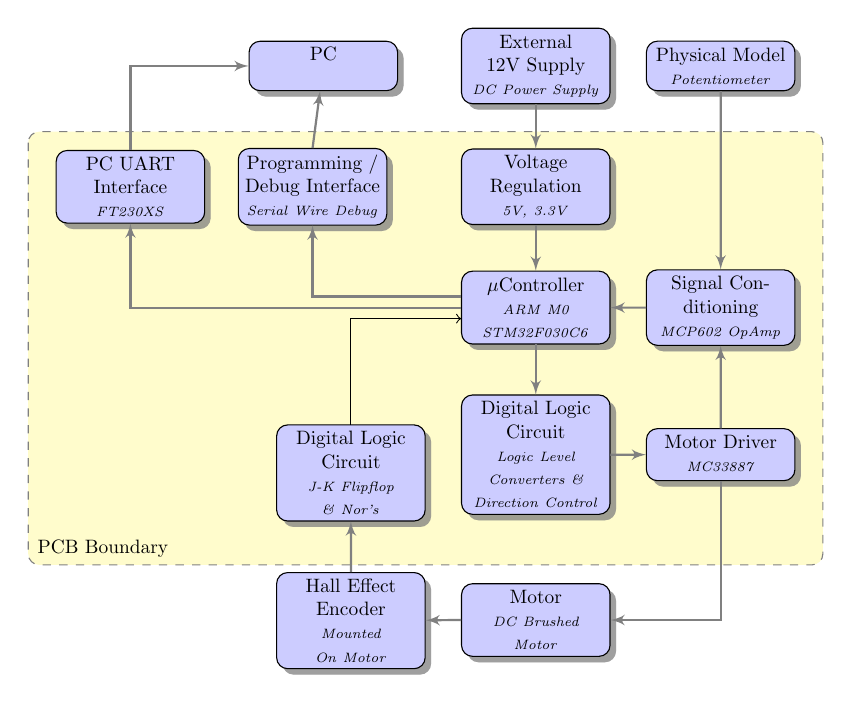
\begin{tikzpicture}[scale=0.7,transform shape]

% Draw diagram elements
\path \external {1}{DC Power Supply};
\path (e1.east)+(2.0,0.0) \physical{1}{Potentiometer};
\path (e1.south)+(0.0,-1.5) \regulator{1}{5V, 3.3V};
\path (r1.south)+(0.0,-1.5) \uC{1}{ARM M0 STM32F030C6};

% PC 
\path (e1.west)+(-2.5,0) \pc{1}{};

% PC UART Interface
\path (r1.west)+(-6,0) \uart{1}{FT230XS};

%Programming/Debug Interface
\path (r1)+(-4.05,0) \prog{1}{Serial Wire Debug};

%Signal Conditioning
\path (uC1.east)+(2.0,0) \sigcond{1}{MCP602 OpAmp};

%JK Flipflops
\path (uC1.west)+(-2.0,-3.0) \encdig{1}{J-K Flipflop \& Nor's};

% Motor
\path (uC1.south) + (0,-5) \motor{1}{DC Brushed Motor};

% Digital Logic: Logic Level Convertes
\path (uC1.south) + (0,-2) \digitlogic{1}{Logic Level Converters \&  Direction Control};

% Motor Driver
\path (digitlogic1.east)+(2.0,0) \motordriver{1}{MC33887};

%Hall Effect Enconder
\path (encdig1.south)+ (0,-1.8) \encoder{1}{Mounted On Motor};




% Draw arrows between elements
\path [line] (e1.south) -- node [above] {} (r1);
\path [line] (r1.south) -- node [above] {} (uC1);

% uC to UART
\path [line] (uC1.west) -| node [below] {} (uart1);

% uC to Programming/Debug Interface
\path [line] (uC1.west)+(0,0.2) -| node [below]{}(prog1); 

% JK FlipFlops
%\path [line] (uC1.west)+(0,-0.2) -| node [above]{}(encdig1); 

\draw[->] (encdig1) |- ([yshift=-0.2cm]uC1.west);


\path [line] (sigcond1.west) -- node[right]{}(uC1);

\path [line] (physical1.south) -- node[above]{}(sigcond1);

% Motor Driver to signal Conditioning
\path [line] (motordriver1.north) -- node[below]{}(sigcond1);

% PC UART Interface -> PC
\path [line] (uart1.north) |- node[left]{}(pc1);

% Programming/Debug Interfac -> PC
\path [line] (prog1.north) -- node[below]{}(pc1);

% Motor Driver -> Motor
\path [line] (motordriver1.south) |- node[right]{}(motor1); 

% Microcontroller -> Digitical logic
\path [line] (uC1.south) -- node[above]{}(digitlogic1);

\path [line] (digitlogic1.east) -- node[left]{}(motordriver1);


\path [line] (encoder1.north) -- node[below]{}(encdig1);


\path [line] (motor1.west) -- node[right]{}(encoder1);

\begin{pgfonlayer}{background}
\path (uart1.west -| physical1.east) node (a) {};
\path (motor1.south -| physical1.south)+(+0.5,-0.3) node (b) {};
\path (digitlogic1.south |- motor1.east)+(+0.5,0.5) node (c) {};

\path[fill=yellow!20,rounded corners, draw=black!50, dashed]
([xshift=-0.5cm,yshift=1cm]uart1.west) rectangle ([xshift=0.5cm,yshift=-2cm]motordriver1.east);           
\path (digitlogic1.north west)+(-0.2,0.2) node (a) {};

\end{pgfonlayer}

\path ([xshift=-4.5cm,yshift=-0.5cm]encdig1.south) node (meep) {PCB Boundary};

 %\path (wa.south)+(0,-\blockdist/5) node (meep) {System Boundary};


\end{tikzpicture}




	
	
\end{document} 